\begin{frame}
\begin{center}
Here is a data type:

\lstinline{Either x (x, x)}
\end{center}
\end{frame}


\begin{frame}
\begin{center}
Algebraically:

\lstinline{x + (x * x)}
\end{center}
\end{frame}


\begin{frame}
\begin{center}
Differentiate

$\frac{\partial}{\partial x}$ \lstinline{(x + (x * x))}
\end{center}
\end{frame}


\begin{frame}
\begin{center}
$\frac{\partial}{\partial x}$ \lstinline{(x + (x * x))}

\tiny{\emph{(sum rule)}}\normalsize{}

\lstinline{=} $\frac{\partial}{\partial x}$ \lstinline{(x +} $\frac{\partial}{\partial x}$ \lstinline{(x * x))}

\tiny{\emph{(power rule, line rule)}}\normalsize{}

\lstinline{= 1 + (2 * x)}

\par\noindent\rule{\textwidth}{0.4pt}

\lstinline{= Maybe (x, x)}
\end{center}
\end{frame}


\begin{frame}
\begin{block}{$\therefore$}
\begin{center}
$\frac{\partial}{\partial x}$ \lstinline{Either x (x, x)}

\par\noindent\rule{\textwidth}{0.4pt}

\lstinline{= Maybe (x, x)}
\end{center}
\end{block}
\end{frame}


\begin{frame}
\begin{block}{$\frac{\partial}{\partial x}$ \lstinline{Either x (x, x)}}
\begin{center}
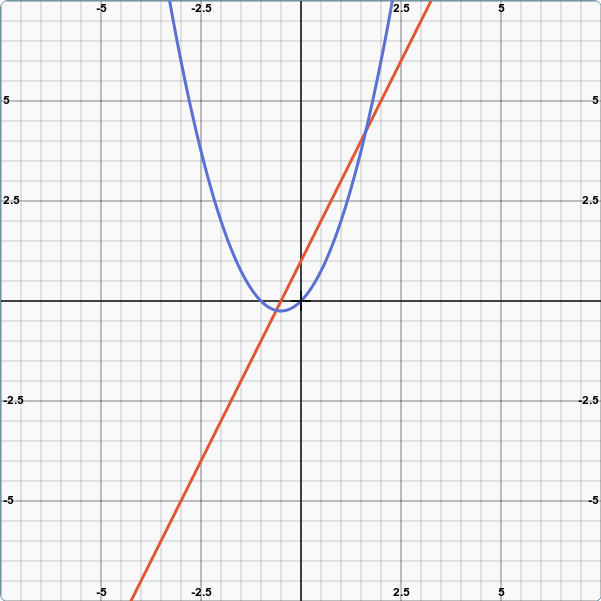
\includegraphics[width=0.75\textheight]{image/derivative_x_plus_x_times_x.png}
\end{center}
\end{block}
\end{frame}


\begin{frame}
\begin{center}
We'll do another one

\lstinline{(Either x x, Either x x)}
\end{center}
\end{frame}


\begin{frame}
\begin{center}
Algebraically:

\lstinline{(x + x) * (x + x)}
\end{center}
\end{frame}


\begin{frame}
\begin{center}
Differentiate

$\frac{\partial}{\partial x}$ \lstinline{((x + x) * (x + x))}
\end{center}
\end{frame}


\begin{frame}
\begin{center}
$\frac{\partial}{\partial x}$ \lstinline{((x + x) * (x + x))}

\lstinline{=} $\frac{\partial}{\partial x}$ \lstinline{4 * x}\textsuperscript{\lstinline{2}}

\tiny{\emph{(power rule)}}\normalsize{}

\lstinline{= 4 *} $\frac{\partial}{\partial x}$ \lstinline{x}\textsuperscript{\lstinline{2}}

\tiny{\emph{(power rule)}}\normalsize{}

\lstinline{= 4 * 2 * x}

\par\noindent\rule{\textwidth}{0.4pt}

\lstinline{= 8 * x}
\end{center}
\end{frame}


\begin{frame}
\begin{block}{$\therefore$}
\begin{center}
$\frac{\partial}{\partial x}$ \lstinline{(Either x x, Either x x)}

\par\noindent\rule{\textwidth}{0.4pt}

\lstinline{= (x, x, x, x, x, x, x, x)}
\end{center}
\end{block}
\end{frame}


\begin{frame}
\begin{center}
A simpler one

\lstinline{(x, x, x)}
\end{center}
\end{frame}


\begin{frame}
\begin{center}
Algebraically:

\lstinline{x * x * x}
\end{center}
\end{frame}


\begin{frame}
\begin{center}
Differentiate

$\frac{\partial}{\partial x}$ \lstinline{x * x * x}
\end{center}
\end{frame}


\begin{frame}
\begin{center}
$\frac{\partial}{\partial x}$ \lstinline{x * x * x}

\lstinline{=} $\frac{\partial}{\partial x}$ \lstinline{x}\textsuperscript{\lstinline{3}}

\tiny{\emph{(power rule)}}\normalsize{}

\lstinline{= 3 *} \lstinline{x}\textsuperscript{\lstinline{2}}
\end{center}
\end{frame}


\begin{frame}
\begin{block}{$\therefore$}
\begin{center}
$\frac{\partial}{\partial x}$ \lstinline{(x, x, x)}

\par\noindent\rule{\textwidth}{0.4pt}

\lstinline{= (Maybe Bool, x, x)}
\end{center}
\end{block}
\end{frame}


\begin{frame}
\begin{center}
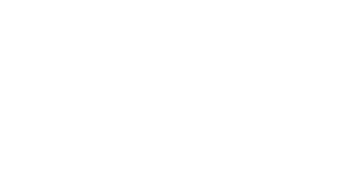
\includegraphics[width=0.3\textheight]{image/crosseyed-blank.png}
\end{center}
\begin{block}{Summary}
\begin{itemize}
  \item \scriptsize{$\frac{\partial}{\partial x}$ \lstinline{Either x (x, x) = Maybe (x, x)}}
  \item \scriptsize{$\frac{\partial}{\partial x}$ \lstinline{(Either x x, Either x x) = (x, x, x, x, x, x, x, x)}}
  \item \scriptsize{$\frac{\partial}{\partial x}$ \lstinline{(x, x, x) = (Maybe Bool, x, x)}}
\end{itemize}
\end{block}
\end{frame}


\begin{frame}
\begin{block}{Insight}
\begin{center}
  The derivative of \emph{any} data structure, \textbf{is its zipper!}\cite{abbott2005data} \footnote{\emph{without the 1-hole context value}}
\end{center}
\end{block}
\end{frame}


\begin{frame}
\begin{center}

\includegraphics[width=0.3\textheight]{image/crosseyed.png}
\end{center}
\begin{block}{Let's stare}
\begin{itemize}
  \item \scriptsize{$\frac{\partial}{\partial x}$ \lstinline{Either x (x, x) = Maybe (x, x)}}
  \item \scriptsize{$\frac{\partial}{\partial x}$ \lstinline{(Either x x, Either x x) = (x, x, x, x, x, x, x, x)}}
  \item \scriptsize{$\frac{\partial}{\partial x}$ \lstinline{(x, x, x) = (Maybe Bool, x, x)}}
\end{itemize}
\end{block}
\end{frame}

\begin{frame}
\begin{block}{Let's do list \tiny{you know you want to}}
\lstinline{List a = 1 + a + a}\textsuperscript{\lstinline{2}} \lstinline{+ a}\textsuperscript{\lstinline{3}} \lstinline{+} \ldots
\end{block}
\end{frame}

\begin{frame}{List}

\lstinline{List a = 1 + a + a}\textsuperscript{\lstinline{2}} \lstinline{+ a}\textsuperscript{\lstinline{3}} \lstinline{+} \ldots

\par\noindent\rule{\textwidth}{0.4pt}

\lstinline{let K a = a + a}\textsuperscript{\lstinline{2}} \lstinline{+ a}\textsuperscript{\lstinline{3}} \lstinline{+} \ldots

\lstinline{List a = 1 + K a}

\emph{\tiny{multiply list by \lstinline{a}}}

\lstinline{K a = a * List a}

\par\noindent\rule{\textwidth}{0.4pt}

{$\therefore$} List a = 1 + a * List a

\emph{\tiny{this makes sense if we think of \lstinline{List} in terms of its constructors}}

\end{frame}


\begin{frame}{List}

\lstinline{List a = 1 + a * List a}

\par\noindent\rule{\textwidth}{0.4pt}

\emph{\tiny{subtract \lstinline{(a * List a)} both sides}}

\lstinline{List a - (a * List a) = 1}

\emph{\tiny{multiply \lstinline{List a} by \lstinline{1}}}

\lstinline{(1 * List a) - (a * List a) = 1}

\emph{\tiny{apply distributive law of multiplication}}

\lstinline{List a * (1 - a) = 1}

\emph{\tiny{divide both sides by \lstinline{1 - a}}}

\lstinline{List a = 1 / (1 - a)}

\par\noindent\rule{\textwidth}{0.4pt}

\emph{\tiny{apply exponent rule}}

{$\therefore$} \lstinline{List a = (1 - a)}\textsuperscript{\lstinline{-1}}

\end{frame}


\begin{frame}{List}

\lstinline{List a = (1 - a)}\textsuperscript{\lstinline{-1}}

\par\noindent\rule{\textwidth}{0.4pt}

\lstinline{let u = 1 - a}

\emph{\tiny{apply chain rule}}

$\frac{\partial}{\partial a}$ {\lstinline{(1 - a)}\textsuperscript{\lstinline{-1}}} \lstinline{=} $\frac{\partial}{\partial u}$ {\lstinline{u}\textsuperscript{\lstinline{-1}}} \lstinline{*} $\frac{\partial}{\partial a}$ \lstinline{1 - a}

\emph{\tiny{differentiate \lstinline{u}\textsuperscript{\lstinline{-1}}}}

$\frac{\partial}{\partial u}$ \lstinline{u}\textsuperscript{\lstinline{-1}} \lstinline{=} \lstinline{-1 / u}\textsuperscript{\lstinline{2}}

\emph{\tiny{differentiate \lstinline{1 - a}}}

$\frac{\partial}{\partial a}$ \lstinline{1 - a} \lstinline{= -1} 

\par\noindent\rule{\textwidth}{0.4pt}

{$\therefore$} $\frac{\partial}{\partial a}$ {\lstinline{(1 - a)}\textsuperscript{\lstinline{-1}}} \lstinline{=} \lstinline{(-1 / u}\textsuperscript{\lstinline{2}}\lstinline{) * -1}

\end{frame}


\begin{frame}{List}

$\frac{\partial}{\partial a}$ {\lstinline{(1 - a)}\textsuperscript{\lstinline{-1}}} \lstinline{=} \lstinline{(-1 / u}\textsuperscript{\lstinline{2}}\lstinline{) * -1}

\par\noindent\rule{\textwidth}{0.4pt}

\emph{\tiny{substitute back \lstinline{u = 1 - a}}}

$\frac{\partial}{\partial a}$ {\lstinline{(1 - a)}\textsuperscript{\lstinline{-1}}} \lstinline{=} \lstinline{(-1 / (1 - a)}\textsuperscript{\lstinline{2}}\lstinline{) * -1}

\emph{\tiny{simplify by multiplying right side by \lstinline{-1}}}

$\frac{\partial}{\partial a}$ {\lstinline{(1 - a)}\textsuperscript{\lstinline{-1}}} \lstinline{=} \lstinline{1 / (1 - a)}\textsuperscript{\lstinline{2}}

\emph{\tiny{apply exponent rule}}

$\frac{\partial}{\partial a}$ {\lstinline{(1 - a)}\textsuperscript{\lstinline{-1}}} \lstinline{=} \lstinline{(1 / 1 - a)}\textsuperscript{\lstinline{2}}

$\frac{\partial}{\partial a}$ {\lstinline{(1 - a)}\textsuperscript{\lstinline{-1}}} \lstinline{=} \lstinline{((1 - a)}\textsuperscript{\lstinline{-1}}\lstinline{)}\textsuperscript{\lstinline{2}}

\par\noindent\rule{\textwidth}{0.4pt}

{$\therefore$} The derivative of a \lstinline{List} is a pair of \lstinline{List}

\end{frame}


\begin{frame}[fragile]
\begin{block}{List derivative}
\begin{lstlisting}[style=haskell]
-- 1 + (a * List a)
List a ~ Nil | Cons a (List a)

-- (1 + (a * List a)) * (1   + (a * List a))
ListDerivative ~ (List a, List a)

-- add the hole back to the derivative
-- (1 + (a * List a)) * a * (1   + (a * List a))
ListZipper ~ (List a, a, List a)
\end{lstlisting}
\end{block}
\end{frame}


\begin{frame}
\begin{center}
\lstinline{data ListZipper a = ListZipper [a] a [a]}
\end{center}

\vspace{1cm}

\begin{center}

\includegraphics[width=0.3\textheight]{image/crosseyed-swirl.png}
\end{center}

\begin{center}
I shall not rob the reader of the fun task of differentiating \lstinline{Tree}

\lstinline{data Tree a = Tree a [Tree a]}

\end{center}

\end{frame}
